%
% fig-1koordinaten.tex
%
% (c) 2025 Prof Dr Andreas Müller
%
\begin{figure}
\centering
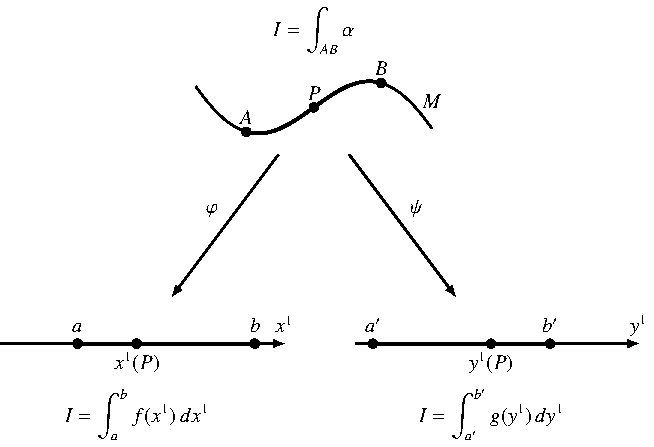
\includegraphics{chapters/030-kurvenintegral/images/1koordinaten.pdf}
\caption{Verschiedene Koordinatensysteme für ein eindimensionales
Definitionsgebiet $M$, auf dem ein Integral berechnet werden soll.
Oben steht ein koordinatensystemunabhängiges Konzept für eine Integral, 
welches in verschiedenen Koordinaten durch ein Riemannsches Integral
berechnet werden kann.
Die Substitutionsformel für das Integral liefert das
Koordinatentransformationsgesetzt zwischen den Darstellungen
$f(x^1)\,dx$ und $g(y^1)\,dy^1$ von $\alpha$.
\label{buch:kurvenintegral:fig:1koordinaten}}
\end{figure}
